\RequirePackage{plautopatch}
\documentclass[uplatex,dvipdfmx,a4paper,11pt]{jlreq}
\usepackage{bxpapersize}
\usepackage[utf8]{inputenc}
\usepackage{fontenc}
\usepackage{lmodern}
\usepackage{otf}
\usepackage{amsmath}
\usepackage{amssymb}
\usepackage{amsthm}
\usepackage{ascmac}
% \usepackage[hyphens]{url}
\usepackage{mhchem}
\usepackage{siunitx}
\usepackage{physics2}
\usephysicsmodule{ab, ab.braket, doubleprod, diagmat, xmat}
\usepackage{diffcoeff}
% \usepackage{braket}
\usepackage{verbatimbox}
\usepackage{bm}
\usepackage{url}
% \usepackage[dvipdfmx,hiresbb,final]{graphicx}
\usepackage{hyperref}
\usepackage{pxjahyper}
\usepackage{tikz}\usetikzlibrary{cd}
\usepackage{tikz-feynhand}
\usepackage{listings}
\usepackage{color}
\usepackage{mathtools}
\usepackage{xspace}
\usepackage{xy}
\usepackage{xypic}
%
\title{原子核物理学}
\author{anko9801}
\makeatletter
%
\DeclareMathOperator{\lcm}{lcm}
\DeclareMathOperator{\Kernel}{Ker}
\DeclareMathOperator{\Image}{Im}
\DeclareMathOperator{\ch}{ch}
\DeclareMathOperator{\Aut}{Aut}
\DeclareMathOperator{\Log}{Log}
\DeclareMathOperator{\Arg}{Arg}
\DeclareMathOperator{\sgn}{sgn}
%
\newcommand{\CC}{\mathbb{C}}
\newcommand{\RR}{\mathbb{R}}
\newcommand{\QQ}{\mathbb{Q}}
\newcommand{\ZZ}{\mathbb{Z}}
\newcommand{\NN}{\mathbb{N}}
\newcommand{\FF}{\mathbb{F}}
\newcommand{\PP}{\mathbb{P}}
\newcommand{\GG}{\mathbb{G}}
\newcommand{\TT}{\mathbb{T}}
\newcommand{\EE}{\bm{E}}
\newcommand{\BB}{\bm{B}}
\renewcommand{\AA}{\bm{A}}
\newcommand{\rr}{\bm{r}}
\newcommand{\kk}{\bm{k}}
\newcommand{\pp}{\bm{p}}
\newcommand{\calB}{\mathcal{B}}
\newcommand{\calF}{\mathcal{F}}
\newcommand{\ignore}[1]{}
\newcommand{\floor}[1]{\left\lfloor #1 \right\rfloor}
% \newcommand{\abs}[1]{\left\lvert #1 \right\rvert}
\newcommand{\lt}{<}
\newcommand{\gt}{>}
\newcommand{\id}{\mathrm{id}}
\newcommand{\rot}{\curl}
\renewcommand{\angle}[1]{\left\langle #1 \right\rangle}
\newcommand{\lbar}{\lambda \kern -0.5em\raise 0.5ex \hbox{--}}
\newcommand\mqty[1]{\begin{pmatrix}#1\end{pmatrix}}
\newcommand\vmqty[1]{\begin{vmatrix}#1\end{vmatrix}}
\numberwithin{equation}{section}

\let\oldcite=\cite
\renewcommand\cite[1]{\hyperlink{#1}{\oldcite{#1}}}

\let\oldbibitem=\bibitem
\renewcommand{\bibitem}[2][]{\label{#2}\oldbibitem[#1]{#2}}

% theorem環境の設定
% - 冒頭に改行
% - 末尾にdiamond (amsthm)
\theoremstyle{definition}
\newcommand*{\newscreentheoremx}[2]{
  \newenvironment{#1}[1][]{
    \begin{screen}
    \begin{#2}[##1]
      \leavevmode
      \newline
  }{
    \end{#2}
    \end{screen}
  }
}
\newcommand*{\newqedtheoremx}[2]{
  \newenvironment{#1}[1][]{
    \begin{#2}[##1]
      \leavevmode
      \newline
      \renewcommand{\qedsymbol}{\(\diamond\)}
      \pushQED{\qed}
  }{
      \qedhere
      \popQED
    \end{#2}
  }
}
\newtheorem{theorem*}{定理}[section]

\newqedtheoremx{theorem}{theorem*}
\newcommand*\newqedtheorem@unstarred[2]{%
  \newtheorem{#1*}[theorem*]{#2}
  \newqedtheoremx{#1}{#1*}
}
\newcommand*\newqedtheorem@starred[2]{%
  \newtheorem*{#1*}{#2}
  \newqedtheoremx{#1}{#1*}
}
\newcommand*{\newqedtheorem}{\@ifstar{\newqedtheorem@starred}{\newqedtheorem@unstarred}}

\newtheorem{sctheorem*}{定理}[section]
\newscreentheoremx{sctheorem}{sctheorem*}
\newcommand*\newscreentheorem@unstarred[2]{%
  \newtheorem{#1*}[theorem*]{#2}
  \newscreentheoremx{#1}{#1*}
}
\newcommand*\newscreentheorem@starred[2]{%
  \newtheorem*{#1*}{#2}
  \newscreentheoremx{#1}{#1*}
}
\newcommand*{\newscreentheorem}{\@ifstar{\newscreentheorem@starred}{\newscreentheorem@unstarred}}

%\newtheorem*{definition}{定義}
%\newtheorem{theorem}{定理}
%\newtheorem{proposition}[theorem]{命題}
%\newtheorem{lemma}[theorem]{補題}
%\newtheorem{corollary}[theorem]{系}

\newqedtheorem{lemma}{補題}
\newqedtheorem{corollary}{系}
\newqedtheorem{example}{例}
\newqedtheorem{proposition}{命題}
\newqedtheorem{remark}{注意}
\newqedtheorem{thesis}{主張}
\newqedtheorem{notation}{記法}
\newqedtheorem{problem}{問題}
\newqedtheorem{algorithm}{アルゴリズム}

\newscreentheorem*{axiom}{公理}
\newscreentheorem*{definition}{定義}

\renewenvironment{proof}[1][\proofname]{\par
  \normalfont
  \topsep6\p@\@plus6\p@ \trivlist
  \item[\hskip\labelsep{\bfseries #1}\@addpunct{\bfseries}]\ignorespaces\quad\par
}{%
  \qed\endtrivlist\@endpefalse
}
\renewcommand\proofname{証明}

\makeatother

\begin{document}
\maketitle
\tableofcontents
\clearpage

\section{原子核}
原子核とは陽子と中性子の集合体である。
この陽子と中性子を核子と呼び、核子は核力や縮退圧を受けながら原子核中を飛び回る。
核反応によって陽子と中性子が互いに遷移し合うような現象や原子核に関する魔法数、ビッグバン時や星の一生でどのように原子核が構成されるかなど、これらをすべて説明するようなモデルを考え、理解するのが原子核物理学である。

\subsection{核子}
陽子と中性子はどちらもスピン 1/2 のフェルミオンである。
\begin{align}
  m_p & = 938.272\ \si{MeV/c^2} \\
  m_n & = 939.565\ \si{MeV/c^2} \\
  m_e & = 0.511\ \si{MeV/c^2}
\end{align}
核子は水素原子の電子と同じような軌道となるのか?

標準核密度 $\rho_0 = 0.17 \si{fm^{-3}}$

魔法数
偶偶核の第一励起状態 21 + の励起エネルギー

フェルミガス模型に従うことから核子が原子核中でかなり自由に動いていることがわかる。


\begin{align}
  d_0 = \frac{a}{E} = \frac{\alpha z Z(\hbar c)}{E}
\end{align}

Woods-Saxon 型分布 (Fermi 関数)
ラザフォード散乱 (Rutherford)
アルファ線 (\ce{^4He} 原子核) を金箔に当てて散乱させた
2万回に1回ほど90度以上の角度に散乱



実験結果、描像、原子核を構成、原子核の性質

原子核の形状因子

密度の飽和性
$r_0 = 1.25 \si{fm}$
\begin{align}
  R = r_0A^{1/3} \\
  4/3\pi R^3 = 4/3\pi r_0^3A
\end{align}
結合エネルギーの飽和性
V0 ≈ 50 MeV,
diffuseness a ≈ 0.53 \si{fm}.
$\rho_0 = 0.17 \si{fm^{-3}}$
\begin{align}
  \rho(r) & = \frac{\rho_0}{1 + \exp(-\frac{r - R}{a})}
\end{align}
電荷 $Ze$
スピン半整数
窒素分子の回転バンドやラマン分光の測定→スピン整数

\subsection{フェルミガス模型}
まずは核子間で相互作用することなく自由に運動しているモデルを考える。 \\
からスピン 1/2 と -1/2 の 2 つがあり、異なるスピンとしか衝突しない。
実際光速の 20 \% 程度で移動している。
陽子や中性子の平均自由行程が長くなる。
統計力学



1 辺 $L$ の立方体の中に $N$ 個の中性子を入れる。
\begin{align}
  \bm{k} = \ab(\frac{2\pi}{L}n_x, \frac{2\pi}{L}n_y, \frac{2\pi}{L}n_z)
\end{align}
\begin{align}
  \psi(\rr) & = e^{i\kk\cdot\rr}
\end{align}

\begin{align}
  dn  & = 4\pi k^2dk \times 2 \ab(\frac{2\pi}{L})^3 = \frac{V}{\pi^2}k^2dk                              \\
  N   & = \int_0^{k_F}\diff{n}{k}\dl{k} = \frac{V}{3\pi^2}k_F^3                                         \\
  k_F & = \ab(\frac{3\pi^2 N}{V})^{1/3}                                                                 \\
  E_F & = \frac{p_F^2}{2m} = \frac{(\hbar k_F)^2}{2m} = \frac{\hbar^2}{2m}\ab(\frac{3\pi^2 N}{V})^{2/3}
\end{align}
\begin{align}
  n   & = 2\int d\rr \int d\pp \frac{1}{h^3} = 2\frac{\Omega}{(2\pi)^3}\int_0^{k_F}4\pi k^2dk = 2\frac{\Omega}{(2\pi)^3}\frac{4}{3}\pi k_F^3 \\
  k_F & = \ab(3\pi^2\frac{n}{\Omega})^{1/3}
\end{align}

\subsection{独立粒子模型}
スピンの影響があるので平均するとよくない。
独立粒子模型がよく成立→平均場近似がよく成立
他の核子からの核力の平均となる場 平均場は Woods-Saxon Potential となる。
1 個の核子の運動に着目 1 粒子軌道
\begin{align}
  V(r) & = -\frac{U_0}{1 + \exp(\frac{r - R}{a})}
\end{align}
Woods-Saxon Potential はシュレーディンガー方程式で解析的に解けないので調和振動子のポテンシャルに近似する。
\begin{align}
  V(r) & = -V_0 + \frac{1}{2}m\omega^2r^2
\end{align}
このとき量子力学でやったように 3 次元極座標系の微分方程式を解くと波動関数 $\psi_{nlm}(\rr) = R_{nl}(r)Y_{lm}(\theta, \varphi)$ に対してエネルギーは次のようになる。
\begin{align}
  H & = -\frac{\hbar^2}{2m}\nabla^2 + \frac{1}{2}m\omega^2r^2 \\
  E & = \ab(2n + l + \frac{3}{2})\hbar\omega
\end{align}
これより $N = 2n + l$ とおくと表 \ref{table:oscillator} のようになる。
\begin{table}[hbtp]
  \centering
  \begin{tabular}{|c|c|c|c|c|c|}
    \hline
    表示 & $N$ & $n$ & $l$ & $m$                & 縮退度 \\
    \hline \hline
    1s & 0   & 0   & 0   & 0                  & 2   \\
    1p & 1   & 0   & 1   & $-1,0,1$           & 6   \\
    1d & 2   & 0   & 2   & $-2,-1,0,1,2$      & 10  \\
    2s & 2   & 1   & 0   & 0                  & 2   \\
    1f & 3   & 0   & 3   & $-3,-2,-1,0,1,2,3$ & 14  \\
    2d & 3   & 1   & 1   & $-1,0,1$           & 6   \\
    \hline
  \end{tabular}
  \caption{調和振動子系の縮退度}
  \label{table:oscillator}
\end{table}
spdfghi

核子が埋まっている
\begin{align}
  \sum_{N = 0}^{N_{max}}(N + 1)(N + 2) = \frac{1}{3}(N_{max} + 1)(N_{max} + 2)(N_{max} + 3) \approx \frac{1}{3}(N_{max} + 2)^3
\end{align}

$N$ ごとに累積和をとると 2, 8, 20, 40, 70

これより平均場近似では魔法数 2, 8, 20, 28, 50, 82, 126 を説明することはできない。

これに対し Mayer, Jensen はスピン軌道結合力を取り入れることで魔法数を説明した。
これが強い理由に軸性ベクトル (擬ベクトル) の話がある
\begin{align}
  V(r) = -V_0 + \underbrace{\frac{1}{2}m\omega^2r^2}_{調和振動⼦} + \underbrace{V_{ls}\bm{l}\cdot\bm{s}}_{スピン軌道結合力}
\end{align}
$V_{ls} = -20A^{-2/3}$ \si{MeV}

\begin{align}
  \langle \bm{l}\cdot\bm{s}\rangle & = \frac{1}{2}[\bm{j}^2 - \bm{l}^2 - \bm{s}^2] = \frac{1}{2} + 1 + 1-
\end{align}

標準核密度 $\rho_0 = 0.17$ \si{fm^{-3}}
\begin{align}
  V(r) = -V_0 + \underbrace{\frac{1}{2}m\omega^2r^2}_{調和振動⼦} + \underbrace{V_{ls}\bm{l}\cdot\bm{s}}_{スピン軌道結合力} + \underbrace{D\bm{l}^2}_{表面項}
\end{align}



\subsection{核の準位}
魔法数 2, 8, 20, 28, 50, 82, 126
により

核子にも準位が存在する。

オープン核
閉殻から核が減っている空孔
閉殻: 全て核⼦が詰まっている = 真空状態
軌道間のエネルギーが数MeVは離れないと閉殻にはなりません。


\subsection{核力}
湯川秀樹によって導入された媒介粒子というアイデアによって
不確定性原理で時間を十分短くするとエネルギーが不確定となる。
これにより短い時間ならエネルギー保存則を破る仮想粒子の交換も実現可能。
$\Delta E = \mu c^2$
\begin{align}
  \Delta t\cdot\Delta E \geq \hbar
\end{align}
核子同士は強い相互作用で束縛されている。
これを核力と呼び、媒介粒子である中間子の交換 (陽子や中性子が中間子をキャッチボール) によって作用される。
核子同士で 1 秒に何回交換されるのか、交換されるときに崩壊は起こるのか?起こるとしたら原子核中のエネルギーはどうなるのか
\begin{align}
  \Delta x = c\Delta t = \frac{\hbar c}{\mu c^2} \approx \frac{197 \si{MeV\cdot fm}}{140 \si{MeV}} \approx 1.4\si{fm}
\end{align}
中間子は $\pi$ 中間子, $\rho$ 中間子, $\omega$ 中間子の 3 つがあり、質量が異なるので、到達距離や結合定数 (⼒の強さ) が変わる。
$\pi$ 中間子は $\pi^+, \pi^-, \pi^0$ の 3 種類がある。
$\pi^\pm$ は弱い相互作⽤ ニュートリノ レプトン数保存
$\pi^0$ は弱い相互作⽤で崩壊しないから電磁気力的に崩壊する。これはとても速く崩壊する。
\begin{table}[hbtp]
  \centering
  \begin{tabular}{|c|c|c|c|c|c|}
    \hline
            & スピン・パリティ & 電荷   & 質量                 & 崩壊寿命                        & 崩壊様式                        \\
    \hline \hline
    $\pi^+$ & $0^-$    & $+e$ & $140$ \si{MeV/c^2} & $2.60\times 10^{-8}$ \si{s} & \ce{\pi^+\to\mu^+ +\nu_\mu} \\
    $\pi^-$ & $0^-$    & $-e$ & $140$ \si{MeV/c^2} & $2.60\times 10^{-8}$ \si{s} & \ce{\pi^-\to\mu^- +\nu_\mu} \\
    $\pi^0$ & $0^-$    & $0$  & $135$ \si{MeV/c^2} & $0.8\times 10^{-16}$ \si{s} & \ce{\pi^0}$\to2\gamma$      \\
    \hline
  \end{tabular}
  \caption{$\pi$ 中間子の種類}
  \label{table:pi}
\end{table}
宇宙線中に観測 (Lattes, Occhialini, Powell, 1947)
加速器(⽶国バークレー、シンクロサイクロトロン)(1948)

\begin{align}
  E^2                 & = (pc)^2 + (mc^2)^2              \\
  \ab(i\diffp{}{t})^2 & = (-i\hbar\nabla c)^2 + (mc^2)^2
\end{align}
定常状態を考えるとコンプトン波長 $\lbar$ を用いて
\begin{align}
   & \ab[\frac{1}{c^2}\diffp[2]{}{t} - \nabla^2 + \ab(\frac{mc}{\hbar})^2]\psi(\rr) = 0                                       \\
   & \ab[\nabla^2 - \frac{1}{\lbar^2}]\psi(\rr) = -4\pi\rho(\rr) = 4\pi g\delta(\rr)    & \ab(\lbar := \frac{\hbar}{m_\pi c}) \\
   & \psi(\rr) = -g\frac{e^{-\frac{r}{\gamma}}}{r}                                                                            \\
   & V(\rr) = -g^2\frac{e^{-r/\gamma}}{r}
\end{align}
中間子場の波動関数は $g$ は核子の持つ荷
核⼦がもつ”荷“が源となって中間⼦場ができると考えます。
の質量が0の時は遠距離⼒、⾮ゼロの時は近距離⼒
\begin{align}
  \alpha = \frac{Z_0 e^2}{2h} = \frac{1}{137} \\
  \frac{g^2}{hc} = 0.3
\end{align}

核⼒ポテンシャル
r,w交換, 2p交換
斥力芯 (クォークパウリ効果等) -0.5fm

\begin{table}[hbtp]
  \centering
  \begin{tabular}{|c|c|c|c|c|}
    \hline
    力     & 重力                             & 電磁気力              & 弱い力                & 強い力                \\
    \hline \hline
    長さ    & $10^8$\si{m} ~ $10^{22}$\si{m} & $10^{-10}$ \si{m} & $<10^{-15}$ \si{m} & $<10^{-15}$ \si{m} \\
    力の大きさ & ~$10^{-38}$                    & ~$10^{-2}$        & ~$10^{-5}$         & ~$1$               \\
    仮想粒子  & 重力子                            & 光子                & W, Z ボソン           & グルーオン (中間子)        \\
    具体例   & 地球-月や銀河系                       & 原子核-電子間           & $\beta$ 崩壊         & 核力                 \\
    \hline
  \end{tabular}
  \caption{自然界の 4 つの力}
  \label{table:force}
\end{table}

荷電交換が起こる確率は 1/2
\begin{figure}[htpb]
  \centering
  \begin{tikzpicture}
    \begin{feynhand}
      \vertex (a) at (0,0); \vertex[particle] (b) at (-1,-1.5){$n$};
      \vertex[particle] (c) at (-1,1.5){$p$};
      \propag[fer] (b) to (a);\propag[fer] (a) to (c);
      \vertex (d) at (1.5,0);
      \propag[photon] (a) to [edge label=$\pi^+$] (d);
      \vertex[particle] (e) at (2.5,1.5){$n$};\vertex[particle] (f) at (2.5,-1.5){$p$};
      \propag[fer] (d) to (e);\propag[fer] (f) to (d);
    \end{feynhand}
  \end{tikzpicture}
  \caption{陽⼦-中性⼦後⽅散乱}
\end{figure}

低エネルギーのp+p,p+n散乱から散乱の位相差
も到達距離(ポテンシャルの形)や引⼒か斥⼒かを評価できます。



\subsection{荷電対称性}
陽⼦と中性⼦の⼊れ替えà物理は変わらない
アイソスピン
\begin{align}
  T = \frac{1}{2}, T_z = -\frac{1}{2} \\
  T = \frac{1}{2}, T_z = +\frac{1}{2}
\end{align}
\begin{align}
  v_n = \begin{pmatrix}
          1 \\ 0
        \end{pmatrix}    \\
  v_p = \begin{pmatrix}
          0 \\ 1
        \end{pmatrix}    \\
  \tau_x = \begin{pmatrix}
             0 & 1 \\
             1 & 0
           \end{pmatrix} \\
  \tau_y = \begin{pmatrix}
             0 & -i \\
             i & 0
           \end{pmatrix} \\
  \tau_z = \begin{pmatrix}
             1 & 0  \\
             0 & -1
           \end{pmatrix} \\
\end{align}

$\Psi = \phi(\rr)\chi(\sigma)v(\tau)$

\subsection{核スピン}
\begin{definition}
  核スピン (原⼦核の全⾓運動量) $J^\pi$
  偶偶核
  基底状態:例外なく全て $J^\pi = 0^+$
  第⼀励起状態:ほとんど $J^\pi = 2^+$
\end{definition}

偶偶核の基底状態はすべて0+です。
奇奇核の場合も基底状態ではあまりないですが、励起状態に0+がある可能性があります。
奇偶核の場合は核スピンは半整数になります。
\begin{align}
  parity = (-)^l
\end{align}

エネルギースケールが違う
超微細構造

原子核の形は Finite Range Liquid Drop Model に従うとされている。ここでは閉殻なら球形、オープン核に核子が多くあるなら楕円形に集団的に変形を引き起こす。
Atomic Data and Nuclear Data Tables,109,1 (2016).
P.Moller, A.J.Sierk, T.Ichikawa, H.Sagawa

歪曲波ボルン近似Distorted-Wave Born Approximation DWBA
平⾯波ボルン近似 Plain-Wave Born Approximation PWBA

\subsection{Fermi 理論}
ニュートリノ (neutrino)

摂動論を用いてフェルミの黄金律 (Fermi' Golden Rule) が導かれる

始状態の波動関数 $\ket|i>$ と終状態の波動関数 $\bra<f|$ 相互作用演算子 $V$
遷移確率 $W$
\begin{align}
  W = \frac{2\pi}{\hbar}|\bra<f|V\ket|i>|^2\diff{N}{E}
\end{align}

\begin{align}
  H = \bra<f|V\ket|i> = g\int(\psi_p^*\tau^-\psi_n)(\psi_e^*\psi_\nu)dt d\rr
\end{align}





\section{原子核の分類と核反応}



\subsection{原子核の構造}
原子は原子核と電子によってできている。
原子核と電子は電磁相互作用で束縛されている。

原子核は核子 (陽子と中性子) によってできている。
原子核の大きさは 1-10fm
元素記号 $X$
質量数 $A$ , 陽子数 $Z$ , 中性子数 $N$ の核種を
\begin{align}
  \ce{^AX}, \ce{^A_ZX}, \ce{^A_ZX_N}
\end{align}

核図表
$r_0 = 1.2 \si{fm}$

Dirac 方程式で元素
電子のエネルギーが虚数
原子核が質点のとき 137
体積があるとき 173
真空崩壊

\begin{itemize}
  \item $A$ が等しい核種を同重体 (isobar)
  \item $Z$ が等しい核種を同位体 (isotope)
  \item $N$ が等しい核種を同中性子体、同調体 (isotone)
  \item $Z$ $N$ が逆の核種を鏡映核 (mirror nuclei)
\end{itemize}

安定核種(安定同位体) ~250種類
発見された核種3312種類 (2020年末時点)
https://people.nscl.msu.edu/~thoennes/isotopes/
6000ー8000種類の原子核の存在が予想
超ウラン元素は核融合によって人工的に生成

強い相互作用によってドリップされる


\subsection{原子核の質量}
陽子と中性子がバラバラになるよりも原子核

原子核の質量は結合エネルギーによって低くなる。低い方へ行く。
核子あたり結合エネルギーは約 $B/A\sim 8$ \si{MeV}
結合エネルギーの飽和性
\ce{^56Fe}

液滴模型のもとで原子の質量を現象論的に表す公式 ヴァイツゼッカーの質量公式 (Bethe-Weizsäcker)
\begin{align}
  M(A, Z) & = ZM(\ce{^1H}) + NM_n - \underbrace{a_VA}_{体積項} + \underbrace{a_SA^{2/3}}_{表面項} + \underbrace{a_C\frac{Z^2}{A^{1/3}}}_{クーロン項} + \underbrace{a_a\frac{(N - Z)^2}{4A}}_{非対称項} + \underbrace{\frac{\delta}{A^{1/2}}}_{対エネルギー項}
\end{align}
陽子数 $Z$ 中性子数 $N$ に対して
\begin{align}
  \delta & = \begin{dcases}
               -\Delta & (A = \mathrm{even}, Z = \mathrm{even}) \\
               0       & (A = \mathrm{odd})                     \\
               +\Delta & (A = \mathrm{even}, Z = \mathrm{odd})  \\
             \end{dcases}
\end{align}
\begin{align}
  a_V    & = 15.67\ \si{MeV/c^2} \\
  a_S    & = 17.23\ \si{MeV/c^2} \\
  a_C    & = 0.714\ \si{MeV/c^2} \\
  a_a    & = 93.15\ \si{MeV/c^2} \\
  \Delta & = 11.2\ \si{MeV/c^2}
\end{align}
\ce{^28O} が⼆重魔法数
安定核の5種(4He,16O,40Ca,48Ca,208Pb )à実験的、理論的に確⽴
不安定核の7種(10He,28O,48Ni,56Ni,78Ni,100Sn,132Sn)、実験的、理論的に確立していないものが
多い。56,78Ni,132Snは実験的、理論的に確立
28Oが難しい理由: 非束縛核(ドリップラインの外)であるため、特に難しい。N/Z比でも突出

体積項
核力は長距離力ではなく近傍の核子からしか引力を受けないから
平均核子間距離 $d = \langle\rho\rangle^{-1/3}$
$A$ は比例

表面項は核表面にいる核子にとっては近傍の核子の数は少ない。体積項の引力を過大評価しているので質量を増やす補正が必要

クーロン項は陽子間のクーロン斥力
これがないと中性子だけで出来た原子核が最も軽く安定になってしまう。

非対称項
陽子と中性子の数が揃っている方が安定
アイソスピン1 (pp, pn, nn) よりもアイソスピン0 (pn) のほうが引力が強い
フェルミ気体模型で分かる

対エネルギー項
陽子数・中性子数がそれぞれ偶数のほうが安定
ともに奇数で安定な核種は \ce{^2_1H_1}, \ce{^6_3Li_3}, \ce{^10_5B_5}, \ce{^14_7N_7} のみ


\subsection{核反応}
安定同位体
$\alpha$ 崩壊
$\beta$ 崩壊
$\gamma$ 崩壊


原子核が他の状態へ遷移する理由は励起状態から基底状態に移ることと質量が軽い方がエネルギーが低く安定だから遷移する。
通常すべて基底状態で核反応時に励起状態になることがある。
核子系はすべて基底状態なのでフェルミガスモデル $T = 0$

ヴァイツゼッカーの質量公式
\begin{align}
  M(A, Z) & = \alpha Z^2 - \beta Z + \gamma + \frac{\delta}{A^{1/2}}
\end{align}
同位体の中で $M(A, Z)$ が極小となるような核種を安定同位体と呼ぶ。
現在知られている最大の安定同位体は \ce{^208Pb}
スズ (錫) : 安定同位体が10種類(最多)
\begin{align}
  Z = \frac{\beta}{2\alpha}
\end{align}
安定同位体に比べて中性子が多ければ $\beta^-$ 崩壊する。
安定同位体に比べて陽子が多ければ $\beta^+$ 崩壊 / 電子捕獲する。
ハイゼンベルクの谷

$\beta^-$ 崩壊は中性子から陽子へ変わる反応 $n \to p + e^- + \overline{\nu}_e$ で $M(A, Z) > M(A, Z + 1)$ のとき起こる。
\begin{align}
  (A, Z) & \to (A, Z + 1) + e^- + \overline{\nu}_e
\end{align}
$\beta^+$ 崩壊は陽子から中性子に変わる反応 $p \to n + e^+ + \nu_e$ で $M(A, Z) > M(A, Z - 1) + 2m_e$ のとき起こる。
\begin{align}
  (A, Z) & \to (A, Z - 1) + e^+ + \nu_e
\end{align}
電子捕獲は電子軌道 (主に K$\alpha$ などの K 殻) の電子と原子核の陽子が反応し, エネルギー $\varepsilon$ の特性 X 線を伴って中性子となる反応 $p + e^- \to n + \nu_e$ で $M(A, Z) > M(A, Z - 1) + \varepsilon$ のとき起こる。
\begin{align}
  (A, Z) + e^- & \to (A, Z - 1) + \nu_e
\end{align}
二重 $\beta$ 崩壊
\begin{align}
  (A, Z) & \to (A, Z + 2) + 2e^- + 2\overline{\nu}_e \\
  (A, Z) & \to (A, Z - 2) + 2e^+ + 2\nu_e
\end{align}
ニュートリノを伴わない二重 $\beta$ 崩壊 ($0\nu2\beta$) があるならニュートリノはディラック粒子 ($\nu \neq \overline{\nu}$) ではなくマヨラナ粒子 ($\nu = \overline{\nu}$) であることがわかる。
⼆重ベータ崩壊はニュートリノがマヨラナ粒子であるか判定する唯⼀の⽅法で \ce{^48Ca}, \ce{^76Ge}, \ce{^124Xe} でよく探索されている。

二重電子捕獲もあり \ce{^78Kr}, \ce{^124Xe}, \ce{^130Ba} に観測例があるがニュートリノレスはまだ。

$\alpha$ 崩壊の条件はなんだろう
鉛より原子番号の大きな放射性同位体でのみ起こりやすい
崩壊前後で質量数を4で割った余りは変化しない

核が励起状態のとき $\gamma$ 崩壊する。



\subsection{Nucleosynthesis}
まずビッグバン元素合成 Big Bang Nucleosynthesis (BBN)

$t\sim 10^{-6}$ \si{s}
$T\sim 1$ \si{GeV} クォーク・グルーオン・プラズマ→ p, n
\begin{align}
  n + \nu_e            & \leftrightarrow p + e^- \\
  p + \overline{\nu}_e & \leftrightarrow n + e^+
\end{align}
これが $1s$ で終わると $p:n \approx 7:1$ に固定される。
\begin{align}
  n + p \leftrightarrow d + \gamma
\end{align}
そして
10分を過ぎると中性⼦の数が減少し、温度も下がりすぎます
中性⼦捕獲が進み

8Beà2 4He, 9Bà8Be+ p
\begin{align}
  \ce{4^1H \to ^4He + 2e^+ + 2\nu}
\end{align}
\ce{3\alpha \to ^12C + \gamma}
ホイル状態
\begin{figure}[htbp]
  \begin{center}
    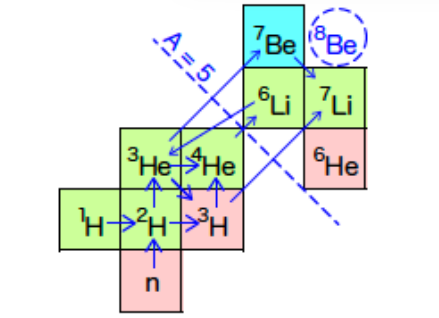
\includegraphics[width=8cm]{./assets/nuclear.png}
    \caption{}
    \label{fig:2level}
  \end{center}
\end{figure}

赤色巨星の一種 AGB 星 (Asymptotic Giant Branch)  sプロセス

r-プロセス (Rapid プロセス)
中性子捕獲の遷移確率 >> ベータ崩壊の遷移確率
中性子星合体または超新星爆発(高密度,高温)
中性子捕獲と光吸収崩壊が平衡化する。
\begin{align}
  \ce{^68Ni} + n & \to \ce{^69Ni} + \gamma                                             \\
  \ce{^69Ni} + n & \to \ce{^70Ni} + \gamma                                             \\
  \ce{^70Ni} + n & \to \ce{^71Ni} + \gamma                                             \\
                 & \vdots                                                              \\
  \ce{^77Ni} + n & \to \ce{^78Ni} + \gamma                                             \\
  \ce{^78Ni} + n & \leftrightarrow \ce{^79Ni} + \gamma \qquad (\textrm{Waiting point})
\end{align}
太陽光のスペクトル+太陽モデル

\section{}


James Chadwick


アイソスピン

\end{document}
